\chapter{HOW TO USE: BR�EL \& KJ�R IMPEDANCE/TRANSMISSION LOSS MEASUREMENT TUBES TYPE 4206}
\label{append-B}

This appendix will cover detailed instructions on the use of the Br�el \& Kj�r Impedance/ Transmission Loss Measurement Tubes Type 4206 and the PULSE data acquisition software.\newline

Determination of normal incidence absorption coefficient and normal specific impedance based on \cite{ISO1998}, \cite{ASTM1990}, and \cite{ASTM2011}.

\begin{center}
    (Warning: Be extremely careful when dealing with the microphone.)
\end{center}
\newpage

\section{Hardware}
This system features the following hardware components:\newline
% Figure 1 here - list of all parts #'d
\begin{figure}[hbtp]
    \centering
    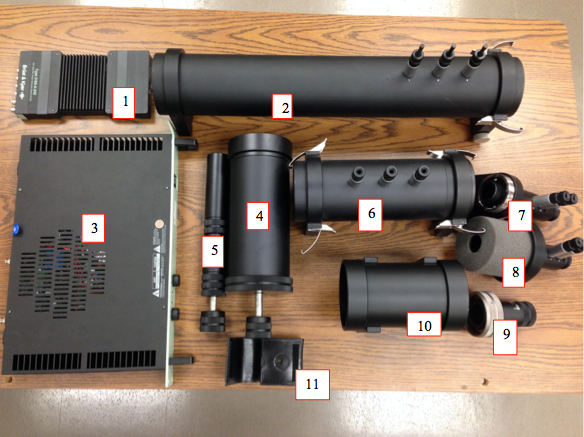
\includegraphics[width=0.9\textwidth]{Appendix-B/figs/allparts}
    \caption{Br�el \& Kj�r Impedance/Transmission Loss Measurement Tubes Type 4206 System}
    \label{fig:allparts}
\end{figure}
% list naming all the parts here
\begin{enumerate}
    \item Data Acquisition Module.
    \item Loudspeaker and large tube.
    \item Power amplifier.
    \item Large tube cap (100mm).
    \item Small tube cap (29mm).
    \item Large tube for microphone 3 and 4 (100mm).
    \item Small tube for microphone 3 and 4 (29mm).
    \item Large to small tube switch.
    \item Small tube sample holder.
    \item Large tube sample holder. 
    \item Microphone Calibrator.
\end{enumerate}

The 100 mm tube is for the frequency range from 50 - 1600Hz.

The 29 mm tube is for the frequency range from 500 - 6300Hz.

\section{Configuring The System}

\subsection{Wiring}
The system features all cables required to properly set up and measure the Transmission Loss or absorption coefficient of a material. Proper wiring can be seen in the figure below.

(Note: Power amplifier should be turned on last prior to an experiment, and turned off first after each experiment.)

% Figure 2 here - wiring of the module and amp
\begin{figure}[hbtp]
    \centering
    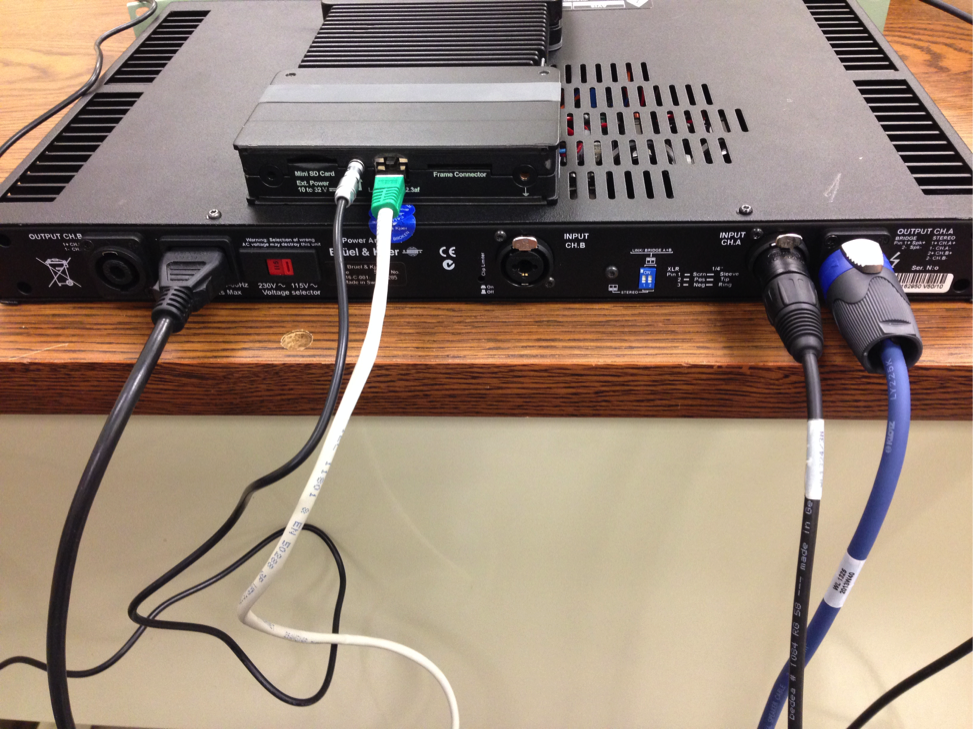
\includegraphics[width=0.8\textwidth]{Appendix-B/figs/modampwire}
    \caption{Wiring of the Module and the Amplifier}
    \label{fig:modampwire}
\end{figure}
% Figure 3 here - wiring of the loud speaker
\begin{figure}[hbtp]
    \centering
    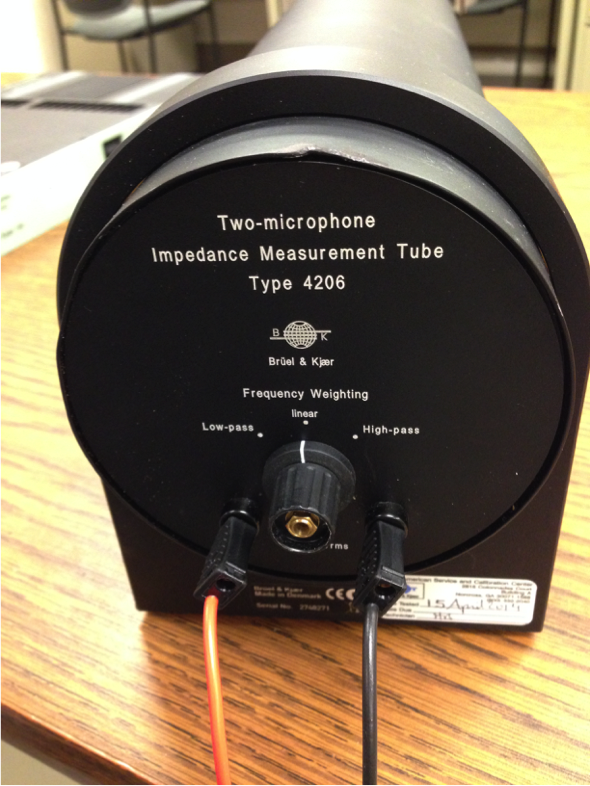
\includegraphics[width=0.6\textwidth]{Appendix-B/figs/loudspeakerwire}
    \caption{Wiring of the Loudspeaker}
    \label{fig:loudspeakerwire}
\end{figure}
\clearpage

The tubes can be configured in two orientations. The first configuration is for measurement of the Transmission loss, and the second configuration is for measurement of the Absorption Coefficient. Each configuration is detailed below.

\subsection{Setting up for Transmission Loss Measurement}

% Figure 4 here - TL set up 
\begin{figure}[hbtp]
    \centering
    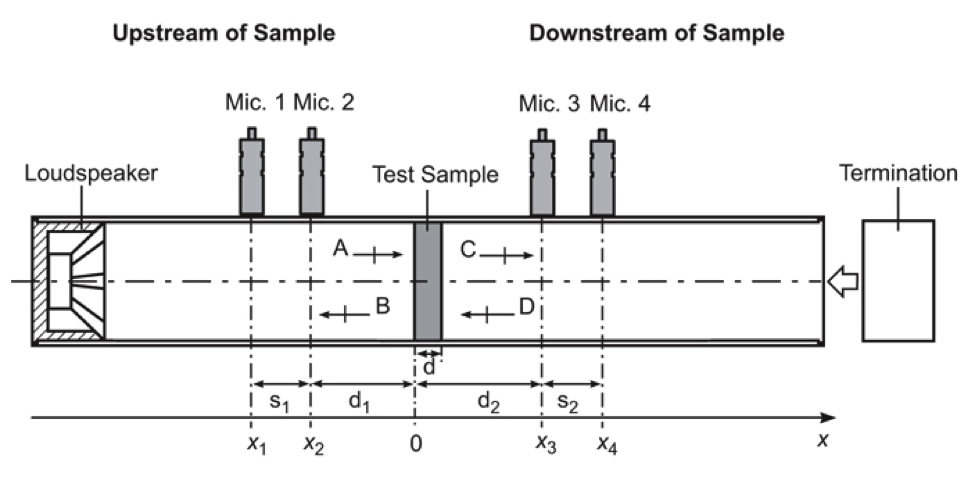
\includegraphics[width=0.7\textwidth]{Appendix-B/figs/TLdiagram}
    \caption{Transmission Loss Diagram}
    \label{fig:TLdiagram}
\end{figure}
\clearpage
For 'Small' tube:
% Figure 5 here - Small Tube TL Wiring w/ Arrows
\begin{figure}[hbtp]
    \centering
    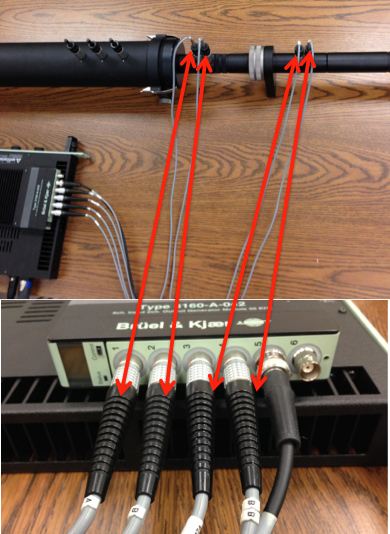
\includegraphics[width=0.6\textwidth]{Appendix-B/figs/TLsmallwirearrows}
    \caption{Transmission Loss Wiring - Small Tube}
    \label{fig:TLsmallwirearrows}
\end{figure}

% Figure 6 here - Small Transmission Tube Sample Location w/ Arrows
\begin{figure}[hbtp]
    \centering
    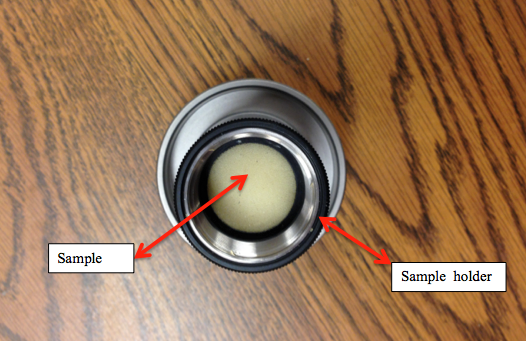
\includegraphics[width=0.7\textwidth]{Appendix-B/figs/TLsmallsample}
    \caption{Transmission Loss - Small Sample Holder}
    \label{fig:TLsmallsample}
\end{figure}
\clearpage
For 'Large' tube:
% Figure 7 here - Large Tube TL Wiring w/ Arrows
\begin{figure}[hbtp]
    \centering
    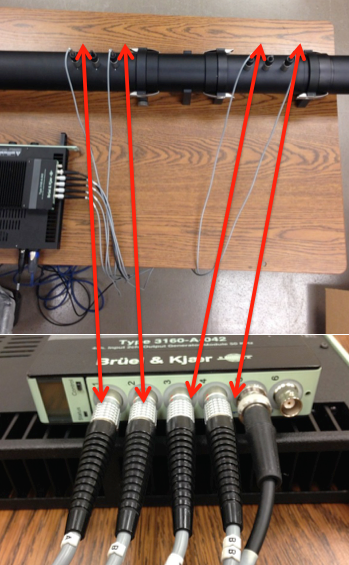
\includegraphics[width=0.5\textwidth]{Appendix-B/figs/TLlargewirearrows}
    \caption{Transmission Loss Wiring - Large Tube}
    \label{fig:TLlargewirearrows}
\end{figure}

% Figure 8 here - Large Transmission Tube Sample Location w/ Arrows
\begin{figure}[hbtp]
    \centering
    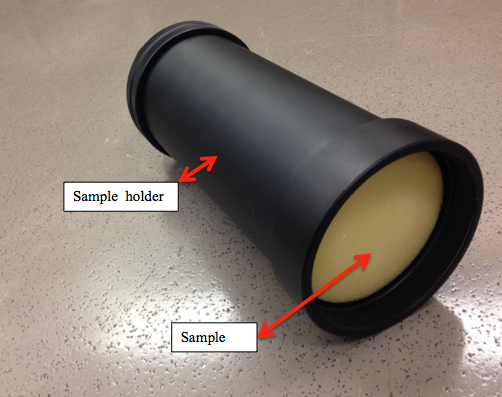
\includegraphics[width=0.7\textwidth]{Appendix-B/figs/TLlargesample}
    \caption{Transmission Loss - Large Sample Holder}
    \label{fig:TLlargesample}
\end{figure}
\clearpage
\subsection{Setting up for Absorption Coefficient Measurement}

To properly measure the Absorption Coefficient of a material, the tubes should be configured as in the figures below.

'Small' tube:
% Figure 9 here - Small Tube Absorption wiring set up
\begin{figure}[hbtp]
    \centering
    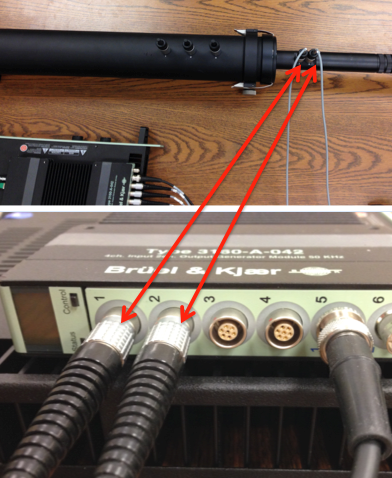
\includegraphics[width=0.6\textwidth]{Appendix-B/figs/Asmallwirearrows}
    \caption{Absorption Coefficient Wiring - Small Tube}
    \label{fig:Asmallwirearrows}
\end{figure}
\clearpage
'Large' tube: 
% Figure 10 here - Large Tube Absorption wiring set up
\begin{figure}[hbtp]
    \centering
    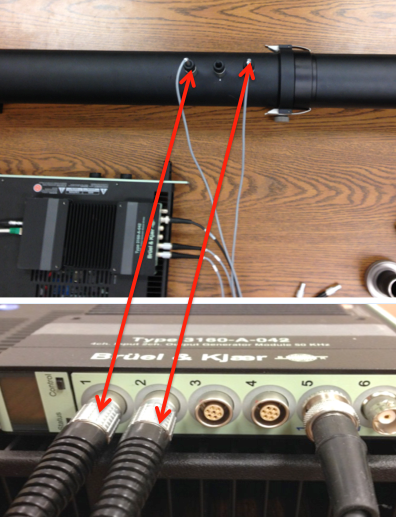
\includegraphics[width=0.6\textwidth]{Appendix-B/figs/Alargewirearrows}
    \caption{Absorption Coefficient Wiring - Large Tube}
    \label{fig:Alargewirearrows}
\end{figure}

\section{Software}
The system uses the provided PULSE software to configure, analyze, collect and export data.

\subsection{Transmission Loss Measurement}
To measure the Transmission Loss of a material begin the PULSE software by opening path:\\
	Start/all program/pulse/applications/Acoustic material testing in tube\\
or click TL Tube on the Desktop.
% Figure 11 here - TL software steps 1 and 2
\begin{figure}[hbtp]
    \centering
    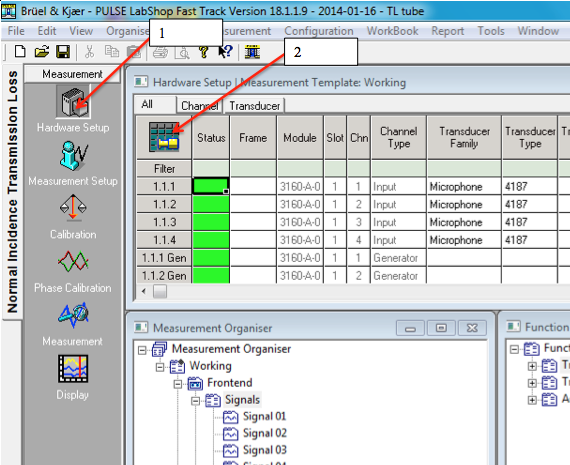
\includegraphics[width=0.5\textwidth]{Appendix-B/figs/TLsoftware12}
    \caption{PULSE Software - Transmission Loss Measurement Steps 1 \& 2}
    \label{fig:TLsoftware1}
\end{figure}
\begin{enumerate}
    \item Click hardware setup on the left, unload the tube.
    \item Then right click chart and select activate template, right click chart again and select auto reconnect.
    If all four microphones are shown as green and connected, go to the next step.
    % Figure 12 here - TL software step 3
    \begin{figure}[hbtp]
        \centering
        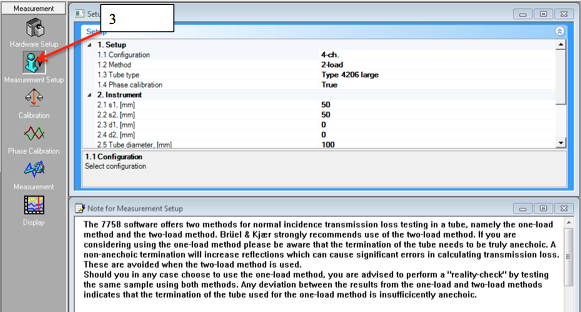
\includegraphics[width=0.7\textwidth]{Appendix-B/figs/TLsoftware3}
        \caption{PULSE Software - Transmission Loss Measurement Step 3}
        \label{fig:TLsoftware3}
    \end{figure}
    \item Click measurement setup 
    \begin{itemize}
        \item Choose 4 ch
        \item Choose 2 load. (means different end, one is with tube, the other one is without)
        \item Tube type depends on the tube
        \item True means you have the phase calibration, false means you do not.
    \end{itemize}
    \clearpage
    % Figure 13 here - repeat of TL diagram
    \begin{figure}[hbtp]
        \centering
        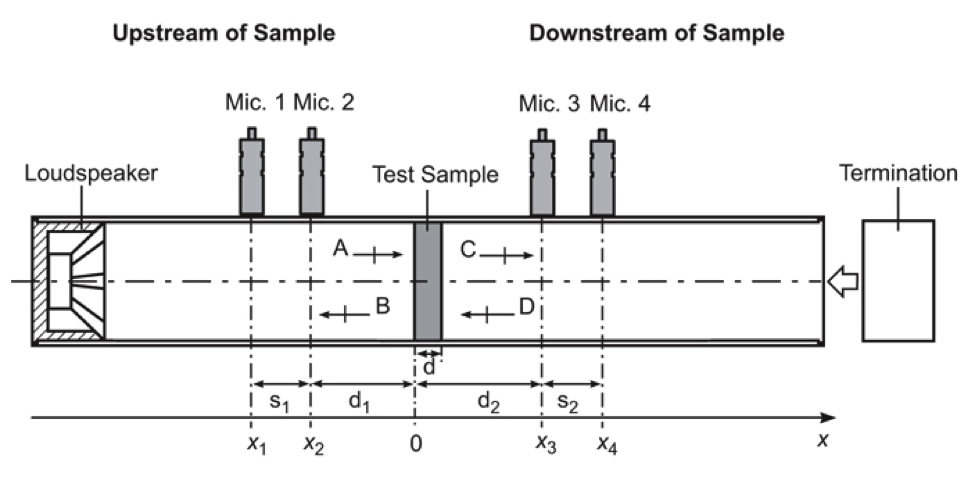
\includegraphics[width=0.6\textwidth]{Appendix-B/figs/TLdiagram}
        \caption{Transmission Loss Diagram}
        \label{fig:TLdiagram}
    \end{figure}
    % Figure 14 here - TL software step 4
    \begin{figure}[hbtp]
        \centering
        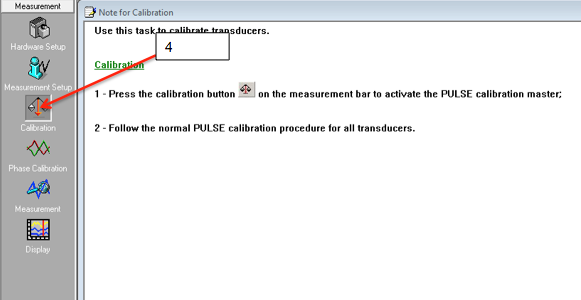
\includegraphics[width=0.6\textwidth]{Appendix-B/figs/TLsoftware4}
        \caption{PULSE Software - Transmission Loss Measurement Step 4}
        \label{fig:TLsoftware4}
    \end{figure}
    \item Calibration of the microphones. 
    Put the microphone into the calibrator, then click calibration, if the result shows green, it means the microphone works well. 
    \clearpage
    % Figure 15 here - TL software step 5
    \begin{figure}[hbtp]
        \centering
        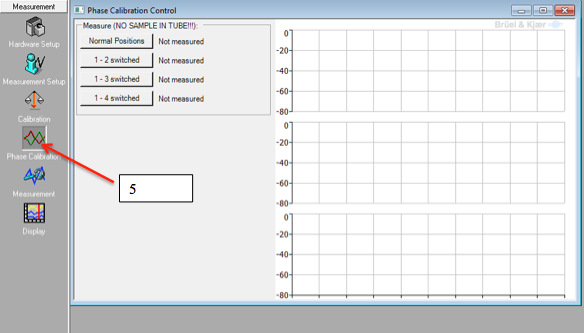
\includegraphics[width=0.6\textwidth]{Appendix-B/figs/TLsoftware5}
        \caption{PULSE Software - Transmission Loss Measurement Step 5}
        \label{fig:TLsoftware5}
    \end{figure}
    \item Click phase calibration, measure the normal position, then follow the commands on the right. When changing the place, perfect out of phase waves should be observed.
    % Figure 16 here - TL software step 6
    \begin{figure}[hbtp]
        \centering
        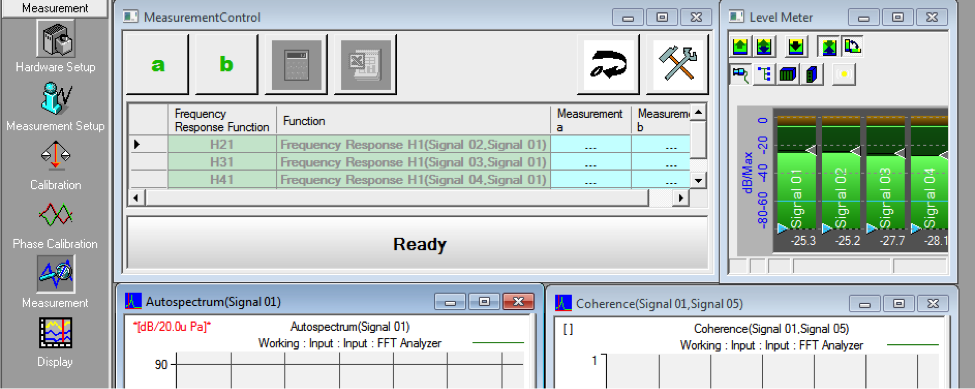
\includegraphics[width=0.6\textwidth]{Appendix-B/figs/TLsoftware6}
        \caption{PULSE Software - Transmission Loss Measurement Step 6}
        \label{fig:TLsoftware6}
    \end{figure}
    \item Load the testing material into the sample holder and click on measurement.
    Click a when the tube end is open and then click b when the tube end is sealed. After measurement click the calculator. Then click export in order to export data into excel. 
        \clearpage
    % Figure 17 here - TL software step 7
    \begin{figure}[hbtp]
        \centering
        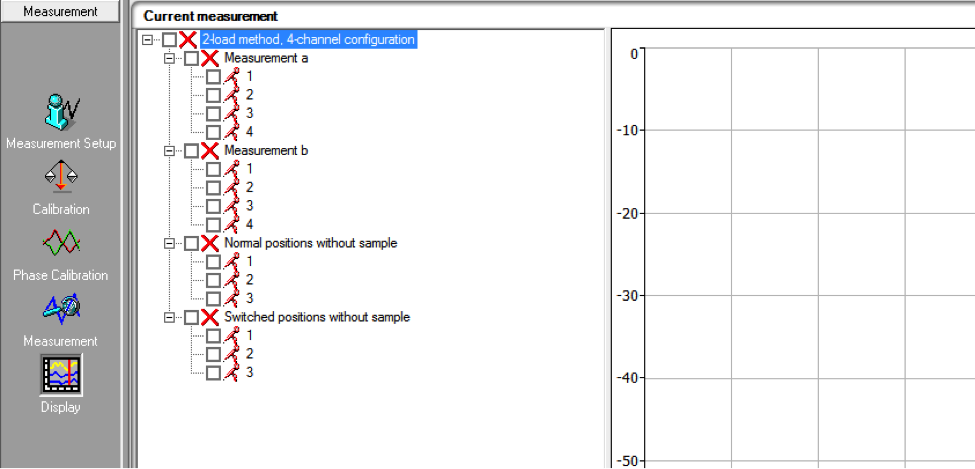
\includegraphics[width=0.7\textwidth]{Appendix-B/figs/TLsoftware7}
        \caption{PULSE Software - Transmission Loss Measurement Step 7}
        \label{fig:TLsoftware7}
    \end{figure}
    \item Click display to have the plot of all the parameters. Check the square of the parameter and drag it to the right to show the figure.
\end{enumerate}
\clearpage
\subsection{Absorption Coefficient Measurement}

To measure the Absorption Coefficient of a material begin the PULSE software by opening path:\\
	Start/all program/pulse/applications/Acoustic material testing in tube\\
or click Absorption Tube on the Desktop.\\

% Figure 18 here - A software steps 1 and 2
\begin{figure}[hbtp]
    \centering
    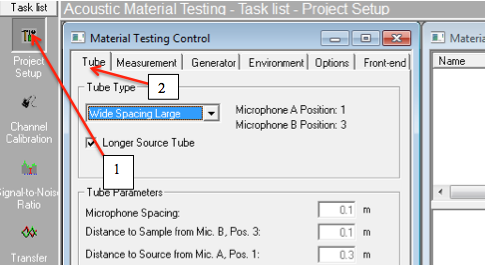
\includegraphics[width=0.7\textwidth]{Appendix-B/figs/Asoftware12}
    \caption{PULSE Software - Absorption Coefficient Measurement Steps 1 \& 2}
    \label{fig:Asoftware12}
\end{figure}
\begin{enumerate}
    \item Click project setup, unload the tube.
    \item Click tube type, choose right type. 
    \clearpage
    % Figure 19 here - A software step 3
    \begin{figure}[hbtp]
        \centering
        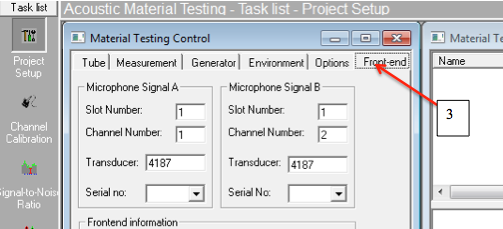
\includegraphics[width=0.6\textwidth]{Appendix-B/figs/Asoftware3}
        \caption{PULSE Software - Absorption Coefficient Measurement Step 3}
        \label{fig:Asoftware3}
    \end{figure}
    \item Click Front-end and change the channel numbers to the numbers displayed above.
    % Figure 20 here - A software step 4
    \begin{figure}[hbtp]
        \centering
        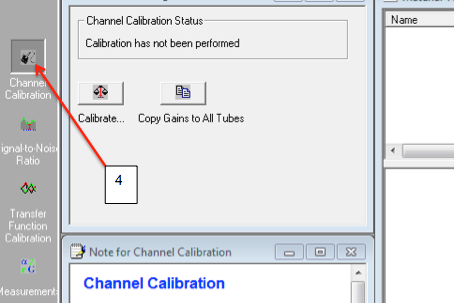
\includegraphics[width=0.6\textwidth]{Appendix-B/figs/Asoftware4}
        \caption{PULSE Software - Absorption Coefficient Measurement Step 4}
        \label{fig:Asoftware4}
    \end{figure}
    \item Click channel calibration, the calibration procedures are the same as in the Transmission loss. 
    \clearpage
    % Figure 21 here - A software step 5
    \begin{figure}[hbtp]
        \centering
        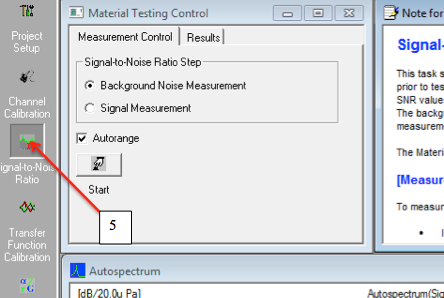
\includegraphics[width=0.7\textwidth]{Appendix-B/figs/Asoftware5}
        \caption{PULSE Software - Absorption Coefficient Measurement Step 5}
        \label{fig:Asoftware5}
    \end{figure}
    \item Click signal to noise ratio, first measure the background noise and press start. Then choose signal measurement, and press start.
    \clearpage
    % Figure 22 here - A software step 6
    \begin{figure}[hbtp]
        \centering
        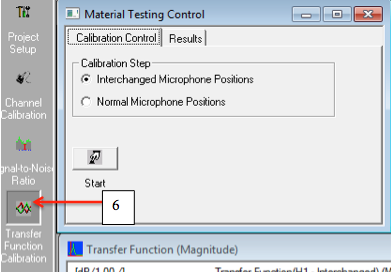
\includegraphics[width=0.7\textwidth]{Appendix-B/figs/Asoftware6}
        \caption{PULSE Software - Absorption Coefficient Measurement Step 6}
        \label{fig:Asoftware6}
    \end{figure}
    \item Click transfer function calibration, and follow the steps in the Transmission loss measurement.
    \clearpage
    % Figure 23 here - A software step 7
    \begin{figure}[hbtp]
        \centering
        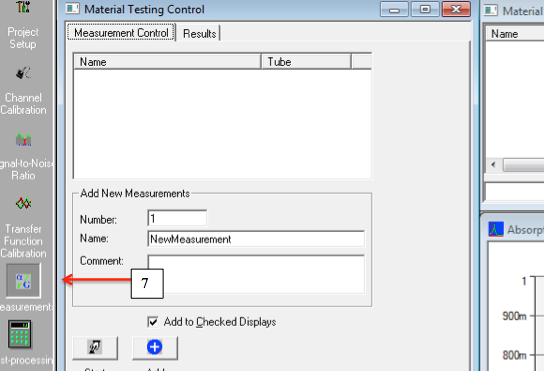
\includegraphics[width=0.7\textwidth]{Appendix-B/figs/Asoftware7}
        \caption{PULSE Software - Absorption Coefficient Measurement Step 7}
        \label{fig:Asoftware7}
    \end{figure}
    \item Load the testing material, and click measurement. Define the test times under number (normally at least 3), and test name under name. Click add to add the test into the task list. Then highlight the one that you want to measure and then click start. Eg:
    % Figure 24 here - A software step 8a
    \begin{figure}[hbtp]
        \centering
        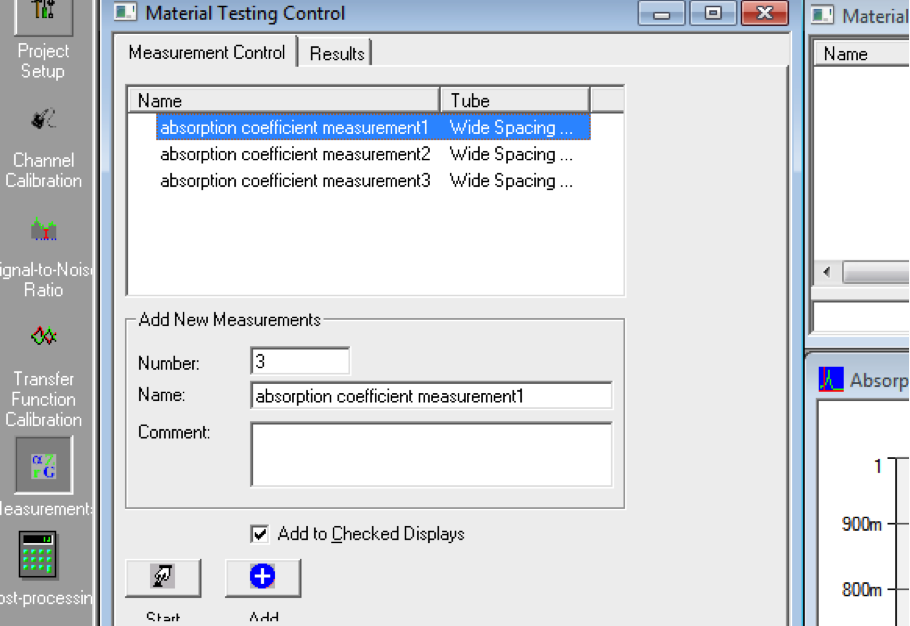
\includegraphics[width=0.7\textwidth]{Appendix-B/figs/Asoftware8a}
        \caption{PULSE Software - Absorption Coefficient Measurement Step 7b}
        \label{fig:Asoftware8a}
    \end{figure}
    \clearpage
    % Figure 25 here - A software step 8b
    \begin{figure}[hbtp]
        \centering
        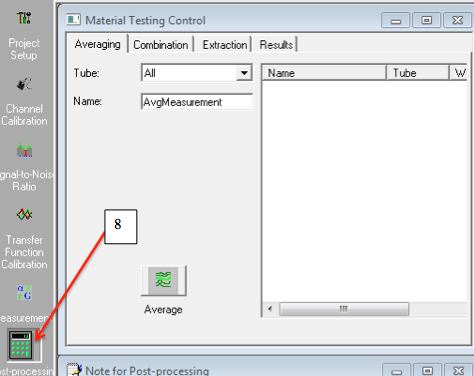
\includegraphics[width=0.7\textwidth]{Appendix-B/figs/Asoftware8b}
        \caption{PULSE Software - Absorption Coefficient Measurement Step 8}
        \label{fig:Asoftware8b}
    \end{figure}
    \item Click post-processing to calculate, in averaging, the tests results can be averaged by checking the small square in front of the test name, in combination, results from the small tube and large tube can be combined together. 
    \clearpage
    % Figure 26 here - A software step 9
    \begin{figure}[hbtp]
        \centering
        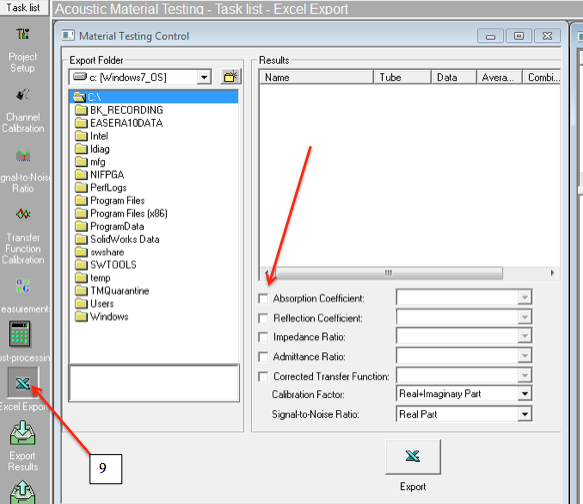
\includegraphics[width=0.7\textwidth]{Appendix-B/figs/Asoftware9}
        \caption{PULSE Software - Absorption Coefficient Measurement Step 9}
        \label{fig:Asoftware9}
    \end{figure}
    \item Click excel export to export the data to excel by checking the squares on the right. Then click export.
\end{enumerate}
